% This conference manuscript template is prepared for:   
% Brian Barrett, Conference Coordinator, Ray W. Herrick Laboratories, Purdue University, West Lafayette, IN, USA. 
% Original version made by Ian H. Bell
% Latest revision = 2021-12-16 by Davide Ziviani 

\documentclass[10pt]{extarticle}
% Miktex users: require l3 packages
%             : optional 3 packages
\usepackage{amssymb,amsmath,multicol,titlesec,apacite,booktabs,tabto,url}
%\usepackage[round]{natbib}  

\usepackage[hmargin = 1in, vmargin = 1in]{geometry}

\renewcommand{\refname}{References}
    
\usepackage[MnSymbol]{mathspec}
\setallmainfonts{Times New Roman}
% Mathspec requires the XeTeX compiler. 

\usepackage[parfill]{parskip}
\usepackage{graphicx}
\usepackage[labelfont=bf]{caption}

\usepackage{titlesec} 
%\titleformat{command}[shape]{format}{label}{sep}{before}[after]
\titleformat{\section}[hang]{\fontsize{12pt}{1em}\selectfont \bfseries}{\thesection. }{0pt}{\centering \MakeUppercase}
\titleformat{\subsection}[hang]{\fontsize{11pt}{1em}\selectfont \bfseries}{\thesubsection}{5pt}{}
\titleformat{\subsubsection}[runin]{}{\thesubsubsection}{5pt}{} 
%\titlespacing{command}{left}{beforesep}{aftersep}[right]
\titlespacing{\section}{0pt}{10pt}{10pt}
\titlespacing{\subsection}{0pt}{10pt}{0pt}
\titlespacing{\subsubsection}{0pt}{10pt}{0pt}	
%\setlength{\bibsep}{3pt}
%\pagenumbering{\gobble}
%\setlength{\hyphenpenalty}{1000}
%\setlength{\exhyphenpenalty}{1000}

\usepackage{fancyhdr}
\pagestyle{fancy}
\fancyhead[R]{\fontsize{12pt}{1em}\selectfont {\textbf {\textit 3\#\#\#}, {\textbf{Page \thepage}}}}
\fancyhead[L]{}
\fancyfoot[C]{7\textsuperscript{th} International High Performance Buildings Conference at Purdue, July 10-14, 2022}
\renewcommand{\headrulewidth}{0pt} % Turn off the bar

%\newcommand\thefontsize[1]{{#1 The current font size is: \f@size pt\par}}

\begin{document}
	
\begin{center}
\vspace{0.2in}
\noindent{\fontsize{14pt}{1em}\selectfont \textbf{Author Instructions to Prepare a Manuscript for the International High Performance Buildings Conference at Purdue 2022}}\\[14pt]

{\fontsize{11pt}{1.2em}\selectfont
First AUTHOR\textsuperscript{1*}, Second AUTHOR\textsuperscript{2}
\\[11pt]
\textsuperscript{1} Organization, Department or Equivalent,\\
City, State, Country\\
Contact Information (Phone, Fax, E-mail)
\\[11pt]
\textsuperscript{2} Organization, Department or Equivalent,\\
City, State, Country\\
Contact Information (Phone, Fax, E-mail)\\[11pt]
* Corresponding Author
\\[33pt]
}
\end{center}

\section*{ABSTRACT}

The first major section of the manuscript is an abstract.  The abstract should describe the contents of the paper, discuss the contribution to the field as well as present the most important results.  Authors are responsible for typing accuracy and proofreading the manuscript.  If accepted, the manuscript must be submitted for reproduction without being edited or retyped by the staff before printing.  The manuscript must look professional and be technically correct in order to be accepted. 

\section{INTRODUCTION}

Each manuscript should begin with an introduction that gives some background on the topic and briefly states the objective of the paper and how it relates to other works in the field.  The manuscripts should report original research or technical developments and their applications.  They should contain quality scientific or technical information.  Manuscripts of a commercial nature will be rejected and will not be authorized for presentation.  The process of acceptance or rejection of papers will be under the authority of the Conference Organizing Committee.  The Organizing Committee will not be held responsible for any errors appearing in the final text.  Authors assume sole responsibility for their manuscript, both for its form and its substance.  Remember to check over the manuscript carefully before submission.  The manuscript should be submitted by only one author. \textbf{Once submitted, no changes to the manuscript will be accepted.} 

\section{HEADINGS FORMAT}

The titles of the main sections have to be centered, numbered and in \textbf{12-point bold type} CAPITAL LETTERS.  With the exception of the abstract, nomenclature, references, and acknowledgments section headings have to be numbered. Blank lines need to be placed above and below each main section title.

\subsection{Sub-Section Headings}
Sub-sections headings have to be in lower case, \textbf{11-point bold type} letters.  A blank line has to be placed above, but not below them.

\subsubsection{Sub-sub-section headings} Sub-sub-sections should be avoided. If they are used, they should be justified left, in normal small letters, with the text beginning to the right.

\section{FORMAT OF THE MANUSCRIPT}

\subsection{Reference Number}
Place the paper ID number at the top right corner of the header in a bold type (for example, ``\textbf{\textit{101}}''); \textit{i.e.}, if you use this template, replace the ``\#\#\#'' in the header of this document with the paper ID number. The paper ID number should be followed by a page number (for example, ``\textbf{\textit{1101}, Page 1}'' for the first page). 

\subsection{Manuscript Title}
Center the manuscript title with font size of \textbf{14-point bolded} with a blank line below the title. 

\subsection{Authors}
All authors should be listed by their full name with the family name appearing last, \textit{i.e.}, how the name is written in English (\textit{e.g.}, Yu Li CHO, John SMITH, Tae-yong KIM). The affiliation of the corresponding author should be given first.  The affiliation and contact information of all co-authors should be listed as well.  When necessary, superscripted numbers should be used to indicate which affiliation corresponds to which author.  The affiliation(s) should be centered and in upper/lower case letters.  The different parts of the affiliation(s) should be separated by commas, and if more than one line is necessary, the different lines should be of about the same length. For manuscripts with multiple authors, an asterisk should be used to identify the corresponding author.  

\subsection{Number of Pages}
The entire manuscript (\textit{i.e.}, text, figures, tables, bibliography, \textit{etc.}) must be no more than ten (10) pages long including graphs, tables and pictures.  Any manuscript having excess pages will not be published. 

\subsection{Text Format}
Times or Times New Roman font type \textbf{MUST} be used for any text in the document including captions, footnotes, and header information.  All text has to be single spaced, black, and in 10-point type. All paragraphs must be single-spaced with a double space between each paragraph. The paragraph format is ``justified''.  If manuscript is prepared in the Asian format, please indicate in Page Set Up ``No Grid Lines''.  Asian single spacing appears as 1-1/2 spacing in Western formats.  Paragraphs are not to be indented. Use single-line spacing between lines except where symbols require 1-1/2 line spaces. 

\subsection{Paper Size and Margins}
Authors are asked to provide the manuscript in 8.5$\times$11 inch standard U.S. letter format following the margin settings explained in this section.  Hardcopy Proceedings will be made available upon request in the 8.5$\times$11 inch standard U.S. letter format.  It is imperative that authors stick to the margin settings.  In order to standardize manuscript presentation, it is important that the procedures listed below be carefully followed. These instructions are also available on the web at \url{https://engineering.purdue.edu/Herrick/Events/Conferences/papers/manuscript-submission}. 

\textbf{IMPORTANT}: All text of the manuscript must be located within a 6.5$\times$9 inch rectangle on a U.S. Standard Letter format page.  The margins are given in Table 1.  An example of the page format is given in Fig. 1.  The \textbf{top margin} has to be set at 1 inch (2.54 cm), the \textbf{left margin} has to be set at 1 inch (2.54 cm), the \textbf{bottom margin} has to be set at 1 inch (2.54 cm), and the \textbf{right margin} has to be set at 1 inch (2.54 cm).  The \textbf{width} of the text should not exceed 6.5 inch (16.5 cm) and the \textbf{length} of the text should not exceed 9 inch (22.87 cm). 

\begin{table}[b]
% Suppressing floating placement of tables/figures in LaTeX is generally deprecated. 
\centering
\caption{Page margins for manuscripts}
\begin{tabular}{ccccc}
\toprule
\textbf{Page Size} & \textbf{Top} & \textbf{Bottom} & \textbf{Left} & \textbf{Right} \\ 
\midrule 
U.S. Standard Letter & 1 inch (2.54 cm) & 1 inch (2.54 cm) & 1 inch (2.54 cm) & 1 inch (2.54 cm) \\ 
\bottomrule 
\end{tabular}
\end{table} 

\subsection{Format of Citations}
Within the text of the manuscript, bibliographical sources are to be cited by giving the last name(s) of the author(s) and the year of publication.  The year should always be in parentheses.  The two possibilities are illustrated as follows:\\
\tabto{0.3in}Albert (1957) showed that the blend was azeotropic.\\
or:\tabto{0.3in}It was shown that the blend was azeotropic (Albert, 1957). 

When there are two authors, the names of both should be cited, \textit{e.g.}:\\
\tabto{0.3in}Albert and Klaus (1981) observed that the blend was azeotropic.\\
or:\tabto{0.3in}It was observed that the blend was azeotropic (Albert and Klaus, 1981). 

When there are three authors or more, only the lead author of the source should be cited. The names of the other authors should be designated by \textit{et al. in italics}, \textit{e.g.}:\\
\tabto{0.3in}Lee \textit{et al.} (1982) observed that the blend was azeotropic.\\ 
or:\tabto{0.3in}It was observed that the blend was azeotropic (Lee \textit{et al.}, 1982). 

When the same author and the same year of publication are cited from more than one source, the sources should be distinguished in the text by adding the small letter ``a'' to the year of publication of the first source cited, ``b'' for the second source, and so on, \textit{e.g.}:\\
\tabto{0.3in}Klaus (1980a) discovered \ldots and further on in the text:\\
or:\tabto{0.3in}Klaus also pointed out (1980b) that \ldots

\emph{Note} that in \LaTeX you can use the citation command, \textit{e.g.}\textbackslash cite$\{$Forbes$\_$1996$\}$, which will show up in the text as \cite{Forbes_1996}. Another example is \cite{Herbe_1997} for a journal article, \cite{Janna_1986} for a book, or \cite{Duminil_1995} for a chapter in a book. The author (year) citations can be typed using the alternative citation command \textbackslash citeA$\{$Forbes$\_$1996$\}$, which will show up in the text as \citeA{Forbes_1996}. 

\subsection{Figures and Tables}
Each table must be numbered (Table 1, 2, 3, \textit{etc.}), with the caption centered above the table and table number in \textbf{bold} as shown in Table 1.  Each figure must be numbered (Figure 1, 2, 3, \textit{etc.}), with the caption centered below the figure and figure number in \textbf{bold} as shown in Figure 1.  Figures and tables should be incorporated into the main body of the text. It is best to position them at the top or bottom of a page and to leave one blank line to separate them from the rest of the text.  Authors have to make sure that all tables and figures appear in their entirety on one page.  All tables and figures must be sharp, clear, AND checked that they are legible in \textbf{black and white}.  All axis and data series must be labeled correctly. All text within the table and diagrams should be in \textbf{English}. The hardcopy proceedings will be black and white.

\begin{figure}
% Suppressing floating placement of tables/figures in LaTeX is generally deprecated. 
\centering
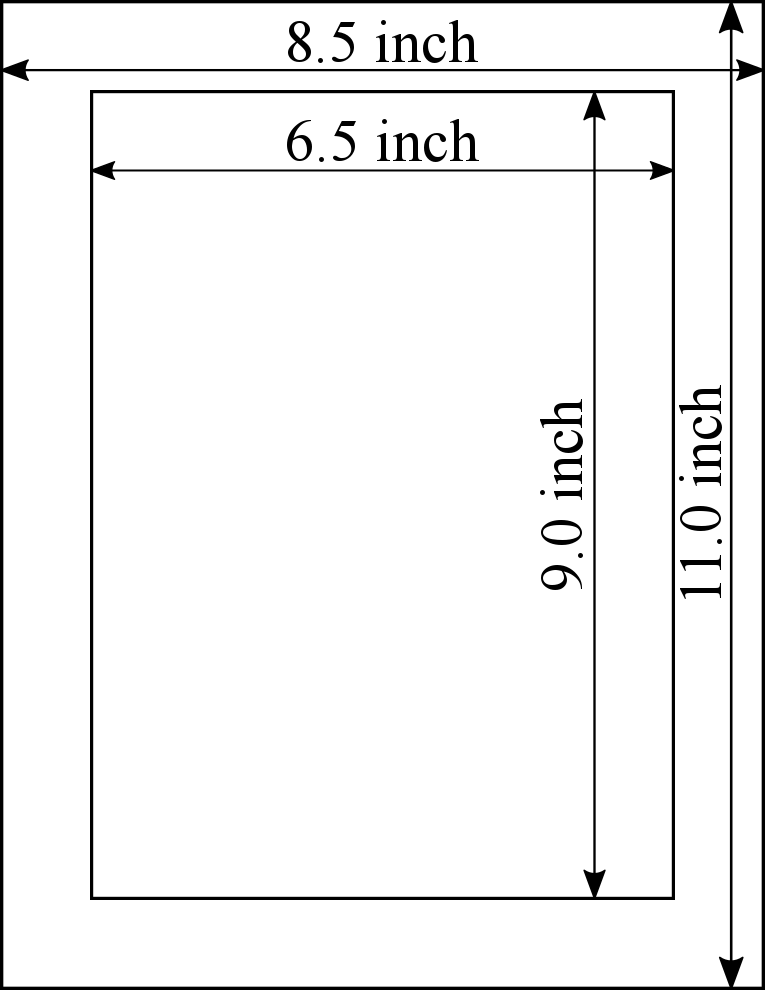
\includegraphics[width = 2.5in]{manuscriptpagesetup}
\caption{Text area for manuscripts (U.S. Letter format)}
\end{figure}

\subsection{Format of Equations}
Equations are to be centered, numbered in order (\textit{i.e.}, (1), (2), (3), \textit{etc.}) down the right-hand side of the page and cited in the text with its number, \textit{e.g.}, ``\ldots as listed in equation (1)''.  Use 1.5 spacing, if necessary, for equations.  

Symbols used in equations should be explained directly below the equation in which they first appear or in a nomenclature section at the end of the manuscript. \textit{E.g.}, a method \cite{Cheap_1986} to estimate the cost of attending meetings is given in Equation (1). Formatting of equations has to be checked before submittal of the manuscript.

\begin{equation}
C = FN_p+AN_n
\end{equation}

\subsection{Units Format}
SI units only or dual units have to be used.  If dual units are used, the equivalent values in the secondary units, enclosed in parentheses, will immediately follow the original values in the primary units, \textit{i.e.}, SI (IP) or IP (SI).

\subsection{Footer and Page Numbering}
Authors are asked to include the one-line footer centered on each page of their manuscript. The footer has to be placed 0.5 inch (1.27 cm) from the bottom edge of the page for the 8.5$\times$11 inch U.S. Standard Letter format.  The required footer is included in the footer of the author template for your conference. The page number should be appended to the paper ID number in the header. 


\section{SUBMISSION OF MANUSCRIPT}

\textbf{DEADLINE}: Submit your manuscripts electronically by \textbf{April 4, 2022} at the online abstract and paper submission website at \textbf{\url{http://www.conftool.com/Herrick2022}}. 

Submit manuscripts as a PDF file that is smaller than 20 MB including an abstract, graphs, and figures.  

\textbf{PUBLICATION OF PAPER}: No manuscript will be published unless the registration fee is paid in full by \textbf{May 30, 2022}.  If your manuscript is rejected, but you are already registered as a required presenting author for the conference, the registration fee will be fully refunded.

\section{COMMERCIALISM}

Commercialization in the manuscript and during the oral presentation is not permitted.  Manuscripts are meant to advance the general state of the art.  The conferences are not a place to promote sales.  If included in the manuscript, \textbf{the paper will either be rejected or the commercialization will be excluded}.  We request, except for the first slide and author identification in the manuscript, that company names, logos and other references to proprietary equipment not be included in the manuscript, on the slides, or in the oral presentation.  However, it is acceptable to describe equipment that was used in experimental tests when necessary for others to be able to reproduce the results.

\section{CONCLUSIONS}

Conclusions can be in paragraph form or bullet items.  Remember the following:

\begin{itemize}
\itemsep-5pt
\item Do not wait until the last minute to submit your paper. 
\item Do not expect to get an extension for submitting your paper. 
\item If you do not submit your paper according to the guidelines specified in these instructions, there is NO GUARANTEE that your paper will be included in the conference proceedings.
\end{itemize}	

\section*{NOMENCLATURE}

The nomenclature should be located at the end of the text using the following format:\\
\begin{samepage}
A\tabto{1.0in}hotel cost\tabto{2.5in}(US\$/night)	\\
C\tabto{1.0in}total cost\tabto{2.5in}(US\$)	\\
F\tabto{1.0in}conference fee\tabto{2.5in}(US\$)\\	
N\tabto{1.0in}number\tabto{2.5in}(–)

\end{samepage}
\begin{samepage}
\textbf{Subscript}\\
n\tabto{1.0in}nights	\\
p\tabto{1.0in}participants
\end{samepage}

\bibliographystyle{apacite}
\bibliography{2020BuildingsTemplate}
\vspace{24pt}
\emph{References} are to be placed at the end of the manuscript in alphabetical order by the last name of the first author.  All sources cited in the text have to be listed in the list of references in alphabetical order of the author's name or of the lead author's name if there are several authors at the end of the manuscript.  The sources should be listed in the standard APA (American Psychological Association) style.  The \texttt{apacite} package will format references in the APA style. 

Examples of APA style citations for other print and electronic sources can be found on the Purdue OWL website, \url{https://owl.english.purdue.edu/owl/resource/560/1/}.

The American Psychological Association maintains a blog where detailed instructions, commentary, and examples for citing different sources are provided: \url{http://blog.apastyle.org/apastyle/}.

Standard abbreviations for periodicals and journals can be found on Web of Science maintained by Thomson Reuters: \url{https://images.webofknowledge.com/WOK46/help/WOS/A_abrvjt.html}.  

\section*{ACKNOWLEDGMENT}

An acknowledgment can be located at the end of the text to indicate the sponsor of the study presented and/or to acknowledge additional contributors to the paper. 

\end{document}
